%%% template.tex
%%%
%%% This LaTeX source document can be used as the basis for your technical
%%% paper or abstract. Intentionally stripped of annotation, the parameters
%%% and commands should be adjusted for your particular paper - title, 
%%% author, article DOI, etc.
%%% The accompanying ``template.annotated.tex'' provides copious annotation
%%% for the commands and parameters found in the source document. (The code
%%% is identical in ``template.tex'' and ``template.annotated.tex.'')

\documentclass[conference]{acmsiggraph}
\usepackage{amssymb}

\TOGonlineid{0}
\TOGvolume{0}
\TOGnumber{0}
%\TOGarticleDOI{1111111.2222222}
\TOGarticleDOI{}
\TOGprojectURL{}
\TOGvideoURL{}
\TOGdataURL{}
\TOGcodeURL{}

\title{Planar Depth Reconstruction for Image Based Rendering}

\author{Puneet Lall\thanks{e-mail:pkl5rc@virginia.edu}\\University of Virginia}
\pdfauthor{Puneet Lall}

%% \keywords{radiosity, global illumination, constant time}

\begin{document}

%% \teaser{
%%   \includegraphics[height=1.5in]{images/sampleteaser}
%%   \caption{Spring Training 2009, Peoria, AZ.}
%% }

\maketitle

% \begin{abstract}

% TODO 

% \end{abstract}

% \begin{CRcatlist}
  % \CRcat{I.3.3}{Computer Graphics}{Three-Dimensional Graphics and Realism}{Display Algorithms}
  % \CRcat{I.3.7}{Computer Graphics}{Three-Dimensional Graphics and Realism}{Radiosity};
% \end{CRcatlist}

% \keywordlist

%% Use this only if you're preparing a technical paper to be published in the 
%% ACM 'Transactions on Graphics' journal.

% \TOGlinkslist

%% Required for all content. 

% \copyrightspace

\section{Introduction}

Image-based rendering provides a practical solution to the task of creating
3D models for rendering of complex scenes, particularly in the case of
novice users who wish to quickly create a visualization of a real-world object.
Rather than requiring users to explicitly create a three-dimensional model using
sophisticated, and often complicated, modeling software, an image-based rendering
system can, for example, 
enable users to render a scene constructed from a sequence of
digital photographs taken by the user.  Thus, such a system can enable
non-expert users to relatively-quickly capture and share a representation of
a three-dimensional scene.
 
Shum and Kang \shortcite{shum2000review} presented a review of various image based
rendering techniques and showed that they can fall onto a spectrum defined
by the representation of their geometric proxy.  While some systems,
such as the Lumigraph \cite{gortler1996lumigraph} allow rendering without
any geometry at all, others use an explicitly-estimated geometrical model
to render.  This work employs the latter approach.

This paper presents a system for reconstructing approximate
piecewise-planar depth-maps for image-based rendering of visualizations
of three-dimensional scenes.  Unlike other image-based rendering systems,
the goal of this work is to create a system which requires relatively few,
unstructured, photographs and can recover dense depth maps with little
processing time.  Furthermore, the recovered geometric representation need
only be accurate enough to enable rendering of a visualization of the depth
of the scene.

Unlike other systems which solve for depth at each pixel,
such as \cite{stuhmer2010real}, this system solves
for a piecewise-planar depth map over a delaunay triangulation
of semi-dense feature points.  Because the selected
semi-dense feature points tend to be located on corners
and gradients, it was found that the resulting triangulation
produces a compact representation which preserves strong
edges in the original image.  Furthermore, unlike the superpixels
used in similar systems, such as \cite{chaurasia2013depth},
the graph of triangular segments this work uses is of uniform degree,
and the resulting geometric proxy is much simpler to render on conventional
rasterization hardware. Furthermore, it ensures a crack-free warp is
achievable without the need to perform costly hole-filling operations.
This is particularly useful for rendering applications which wish to
run on modern mobile devices with limited hardware acceleration capabilities.
In addition, solving for the geometric proxy directly, as opposed to 
reconstructing a dense depth map only to later simplify the proxy geometry
before rendering, eliminates redundant computation of precise measurements
only to be discarded.

Finally, the system requires little processing time compared
to dense reconstruction methods such as \cite{furukawa2010accurate}.
Although the reconstruction is much less accurate and significantly simpler,
in that it is constrained to a single depth-map and cannot reconstruct
geometry occluded in the primary view,
the results appear to be adequate for image-based rendering of compelling depth
visualizations.

\section{Approach}

The implemented system for depth reconstruction takes, as input, a sequence
of images captured by hand at roughly the same orientation, but at varying
translational offset.  The system then reconstructs a depth map for the
first image in the sequence, the primary image, based on the additional
viewpoints provided by the rest of the images in the sequence,
referred to as secondary images.
To reconstruct depth, a structure-from-motion
procedure is first employed to simultaneously estimate the depth of several
sparse points in the scene as well as the pose of the camera
for each secondary image relative to that of the camera in the primary image.
Then, a more dense set of keypoints are used to 
estimate a piecewise-planar approximation of the depth map
via fusion of depth samples from the various secondary images using
a probabilistic model.
Finally, a relief-like representation of the scene geometry is rendered
with hardware-acceleration using OpenGL.

\subsection{Structure from Motion}

Before a dense depth map can be recovered via multi-view stereo,
extrinsic camera parameters, namely translation and rotation, must be known.
To estimate this, a structure from motion algorithm similar to that
described in \cite{snavely2006photo} was implemented to
simultaneously solve for the camera pose for each secondary image,
relative to the primary image.
Unlike \cite{snavely2006photo}, however, since we are concerned
only with the depth of points relative to the primary image,
points in the scene are assumed to be exactly co-linear with
their projection in the primary image.  Thus, instead of having
to estimate three parameters, x, y and z for each point,
only a single depth must be computed.  Furthermore, the use
of a primary view also simplifies the handling of occlusion throughout
the pipeline such that pruning of occluded feature points
is not necessary since we are only concerned with points which
are visible in the primary image.

The structure from motion algorithm begins by finding good feature points
to track between images.  The algorithm of \cite{shi1994good}, as implemented
in \cite{opencv_library}, is used to find good features to track in the
primary image.
Furthermore, a uniform, square grid is superimposed over the image and only
the optimal feature point in each cell is used.
The KLT feature tracking algorithm is then used to find the points in each
secondary image corresponding to the feature point in the primary image.

Once sparse point correspondences have been found, a RANSAC procedure
is used to estimate the fundamental matrix relating each secondary
image to the primary image.  Outlier correspondences are discarded at this
stage, and secondary images are sorted by order of the number of inlier
correspondences found such that those with the most inliers will
be processed first in the next stage.  Also, secondary images containing
too few inlier correspondence points, relative to a pre-determined
threshold, are discarded as outliers.  Note, too, that correspondence
points are transformed, prior to fundamental-matrix estimation, to normalized
device coordinates, assuming that the camera has its optical center at the center of each
photograph and also has no skew.  Thus, the estimated fundamental matrix
can be used as the essential matrix for the image pair since
we are only concerned with reconstructing depth up to a constant scale
factor and all images are assumed to have been captured with the
same focal length.

An initial set of depth values associated with sparse features in
the primary image are determined from the first secondary image
to be processed as follows.  First, the relative pose of this secondary
image is determined by the previously-estimated essential matrix via
singular-value-decomposition and the method of \cite{hartley2003multiple}.
This pose can only be determined up to an ambiguity of four candidate poses,
so a simple voting procedure is used whereby the selected candidate pose is
that which maximizes the number of tracked points which, when triangulated,
are in front of both cameras.  Triangulation is performed according to the
method discussed in \cite{hartley1997triangulation}.  Finally, points
for which triangulated depth is negative relative to either camera
are discarded as outliers.

Next, the system involving sparse triangulated points and the secondary
image's relative camera pose is optimized using the sparse-bundle-adjustment
framework of \cite{ceres-solver}.  Specifically, given a set of depth values,
$\{d_0, ..., d_n\}$, corresponding to keypoints with observations in the
primary image, $\{(x_0^0, y_0^0), ..., (x_n^0, y_n^0)\}$, and observations
in a secondary image, with index $i \in \{0, ..., m\}$, denoted as
$\{(x_0^i, y_0^i), ..., (x_n^i, y_n^i)\}$, the energy to minimize is
given by

\begin{equation}
    \label{eq:sfm}
    E = \sum_{i=0}^{m} \sum_{j=0}^{n}
    \rho \left(
    \begin{pmatrix}
        x_i^j\\
        y_i^j
    \end{pmatrix}
    -
    \pi_j
    \begin{pmatrix}
        x_i^0 d_0\\
        y_i^0 d_0\\
        d_0
    \end{pmatrix}
    \right)
\end{equation}

where $\pi_i$ indicates the projection of a point in $\mathbb{R}^3$ onto
the projection plane of the $i$th camera and
$\rho$ is the Huber loss function, \cite{huber1964robust}, applied component-wise
to the projection residual vector.  Note that the use of the robust Huber loss
function is critical to reduce sensitivity to outliers.

The remaining secondary images are added to the system one-by-one
by first estimating their pose via a RANSAC-like procedure.
Three correspondences with existing depth estimates are randomly selected,
and then the camera pose, defined by translation and a rotation quaternion,
which reduces the energy given in (\ref{eq:sfm}) using a squared loss-function
in place of the Huber loss function is determined using the levenberg-marquardt
solver of \cite{ceres-solver}.  Finally, the pose with the minimum global
energy, computed over all correspondences, is selected and refined,
again using levenberg-marquardt to minimize the energy (\ref{eq:sfm}) while
keeping depth values fixed.  
One pose is estimated, additional correspondence points are triangulated,
and the sparse bundle-adjustment procedure is performed again to refine
the system.  Figure~\ref{fig:initial_depth} shows the resulting sparse depth
samples recovered for an image sequence.

\begin{figure}[ht]
  \centering
  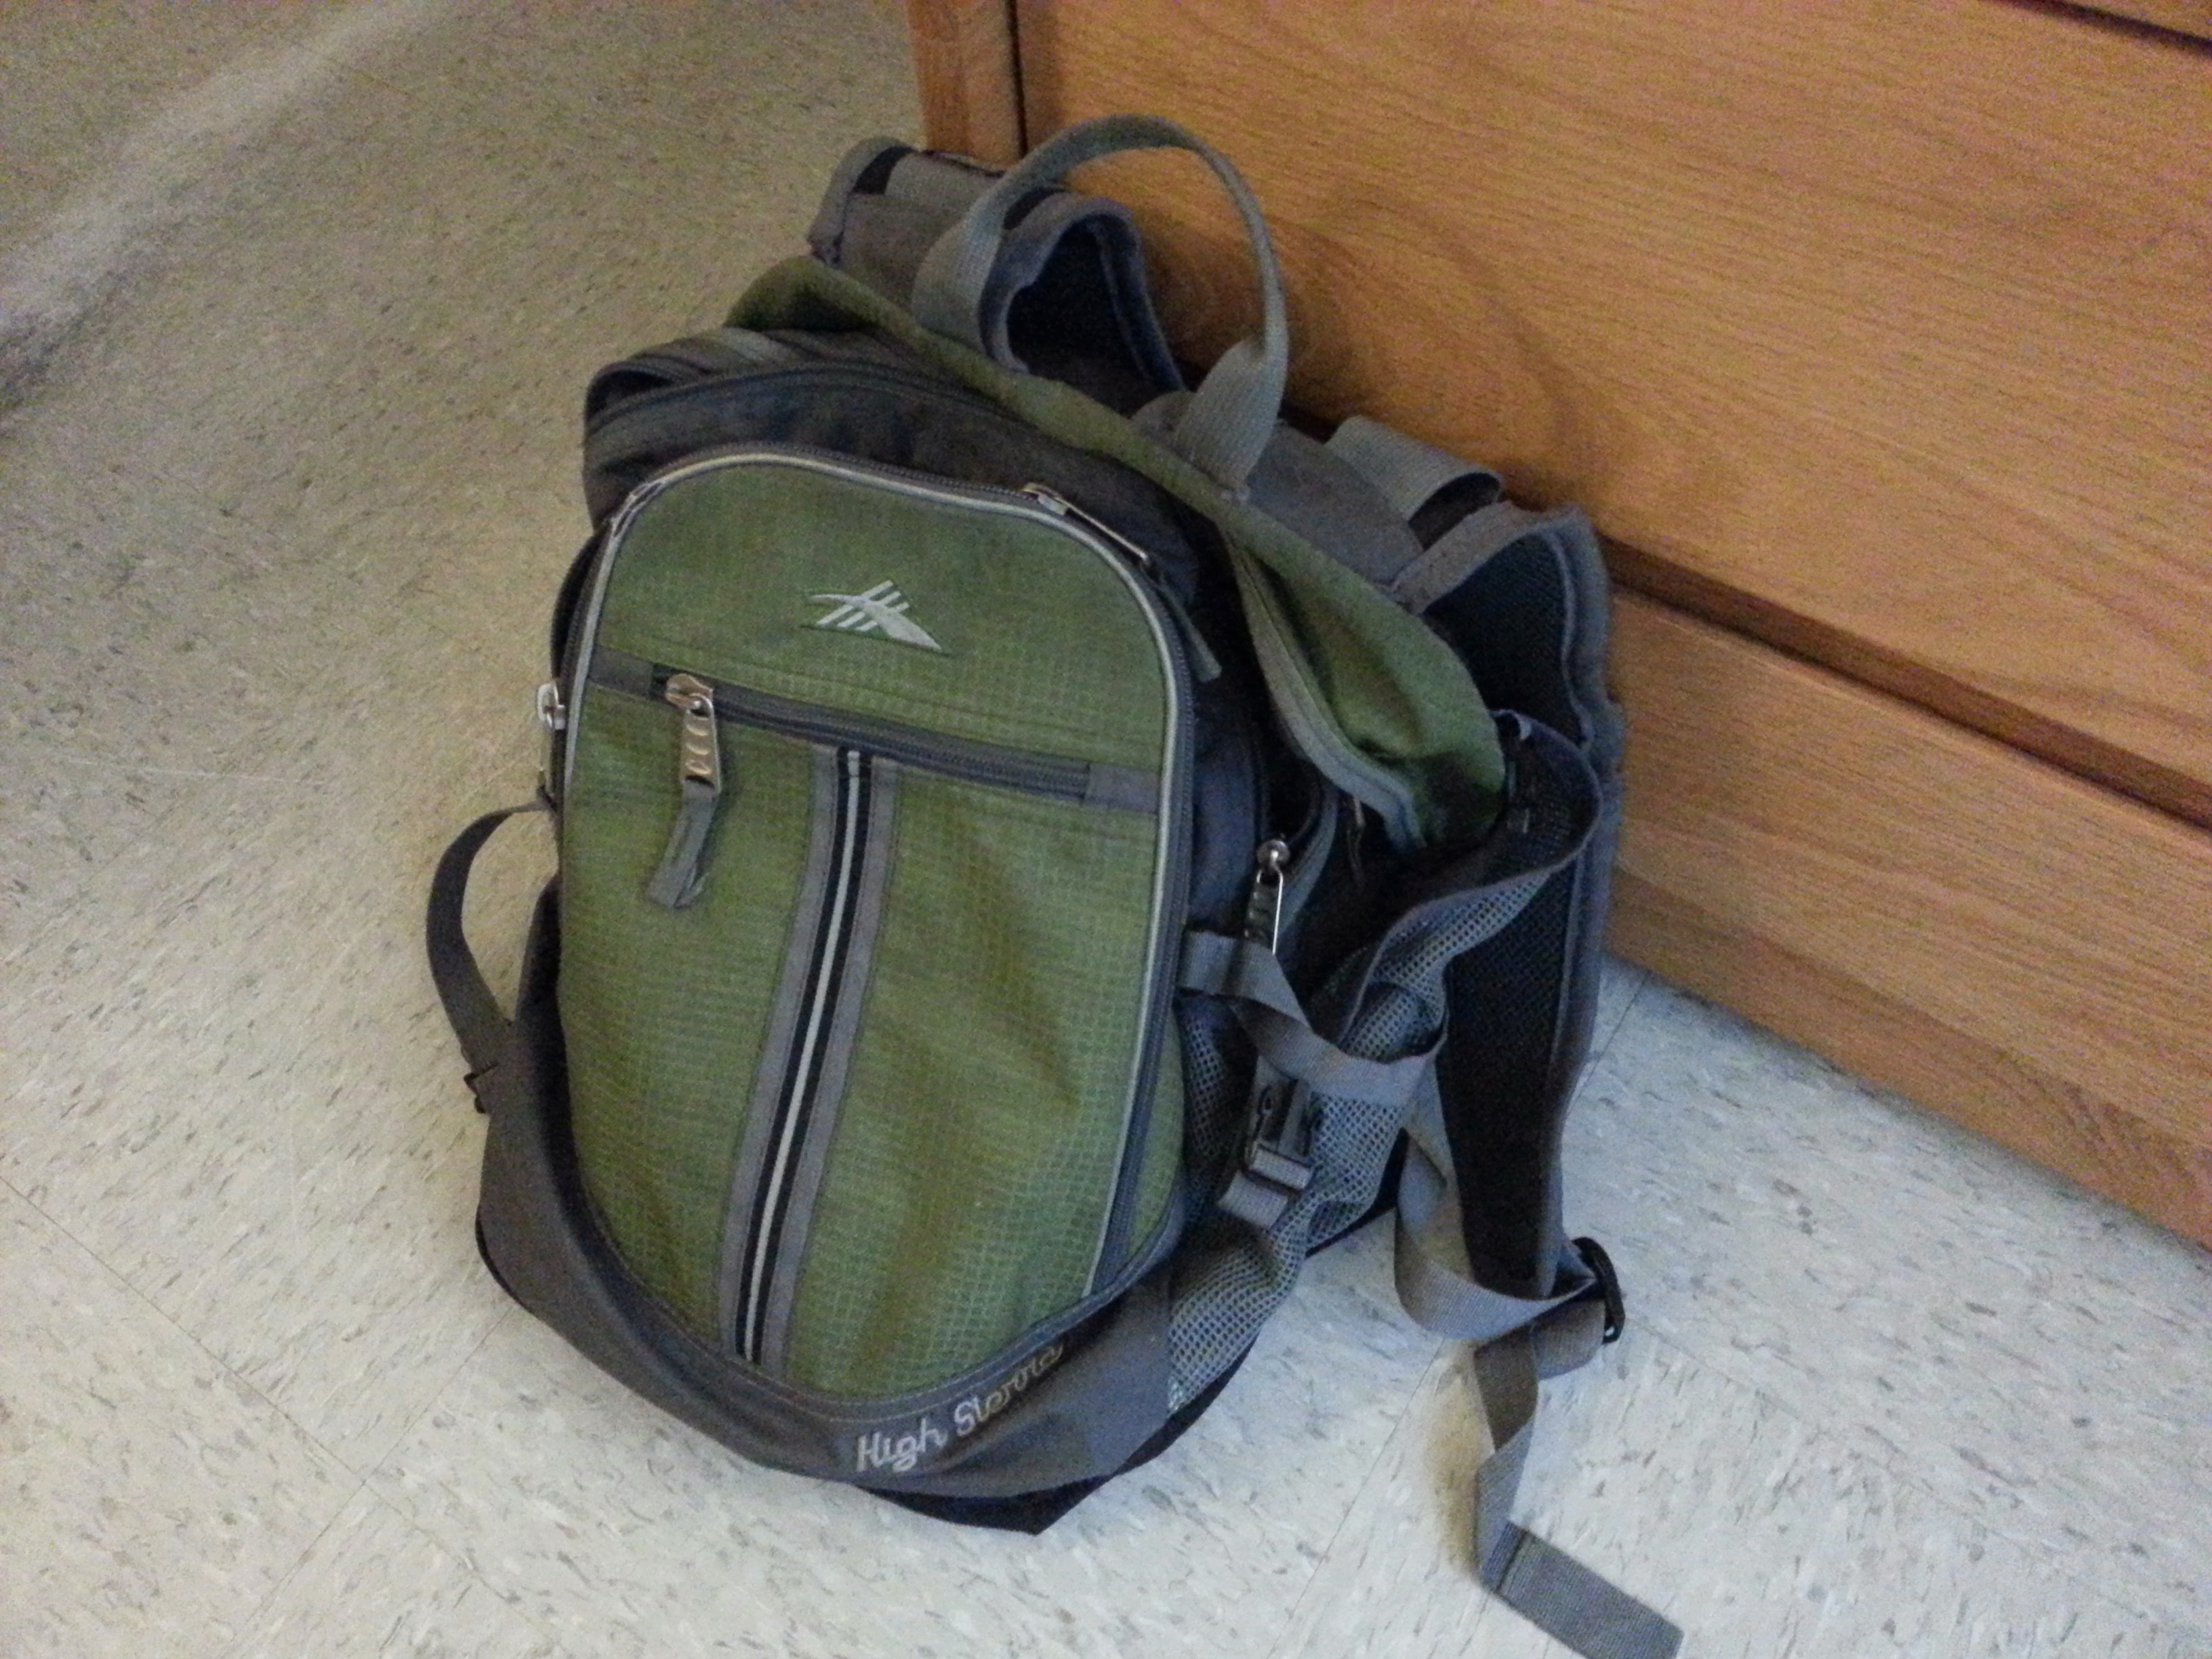
\includegraphics[width=3in]{images/backpack}
  \caption{The primary image from a sequence of images.}
  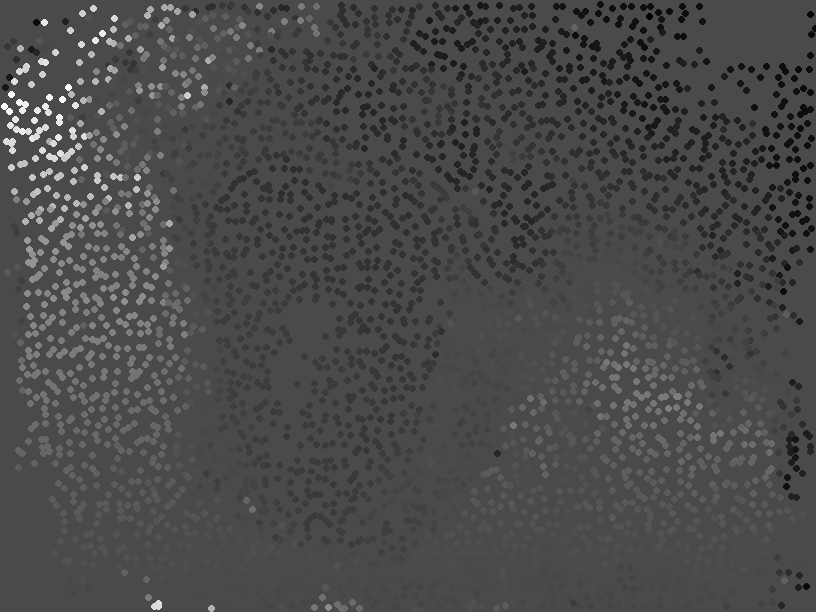
\includegraphics[width=3in]{images/initial_depth}
  \caption{Sparse depth estimates resulting from structure-from-motion. Brighter
  dots indicate greater distance from the camera.}
  \label{fig:initial_depth}
\end{figure}

\subsection{Depth Reconstruction}

% TODO show images of each step

The previously-discussed structure-from-motion process recovers
only a very sparse set of depth samples which is inadequate
for the intended rendering application.
To compute a more dense set of depth samples, additional KLT feature
correspondences are matched using the same procedure as before.
In the results displayed below, 20 thousand points are used.
Instead of adding these to the structure-from-motion problem,
which would result in a slower process, a probabilistic
approach is used to merge candidate depth samples
to solve for a plausible piecewise-planar depth map.

\begin{figure}[ht]
  \centering
  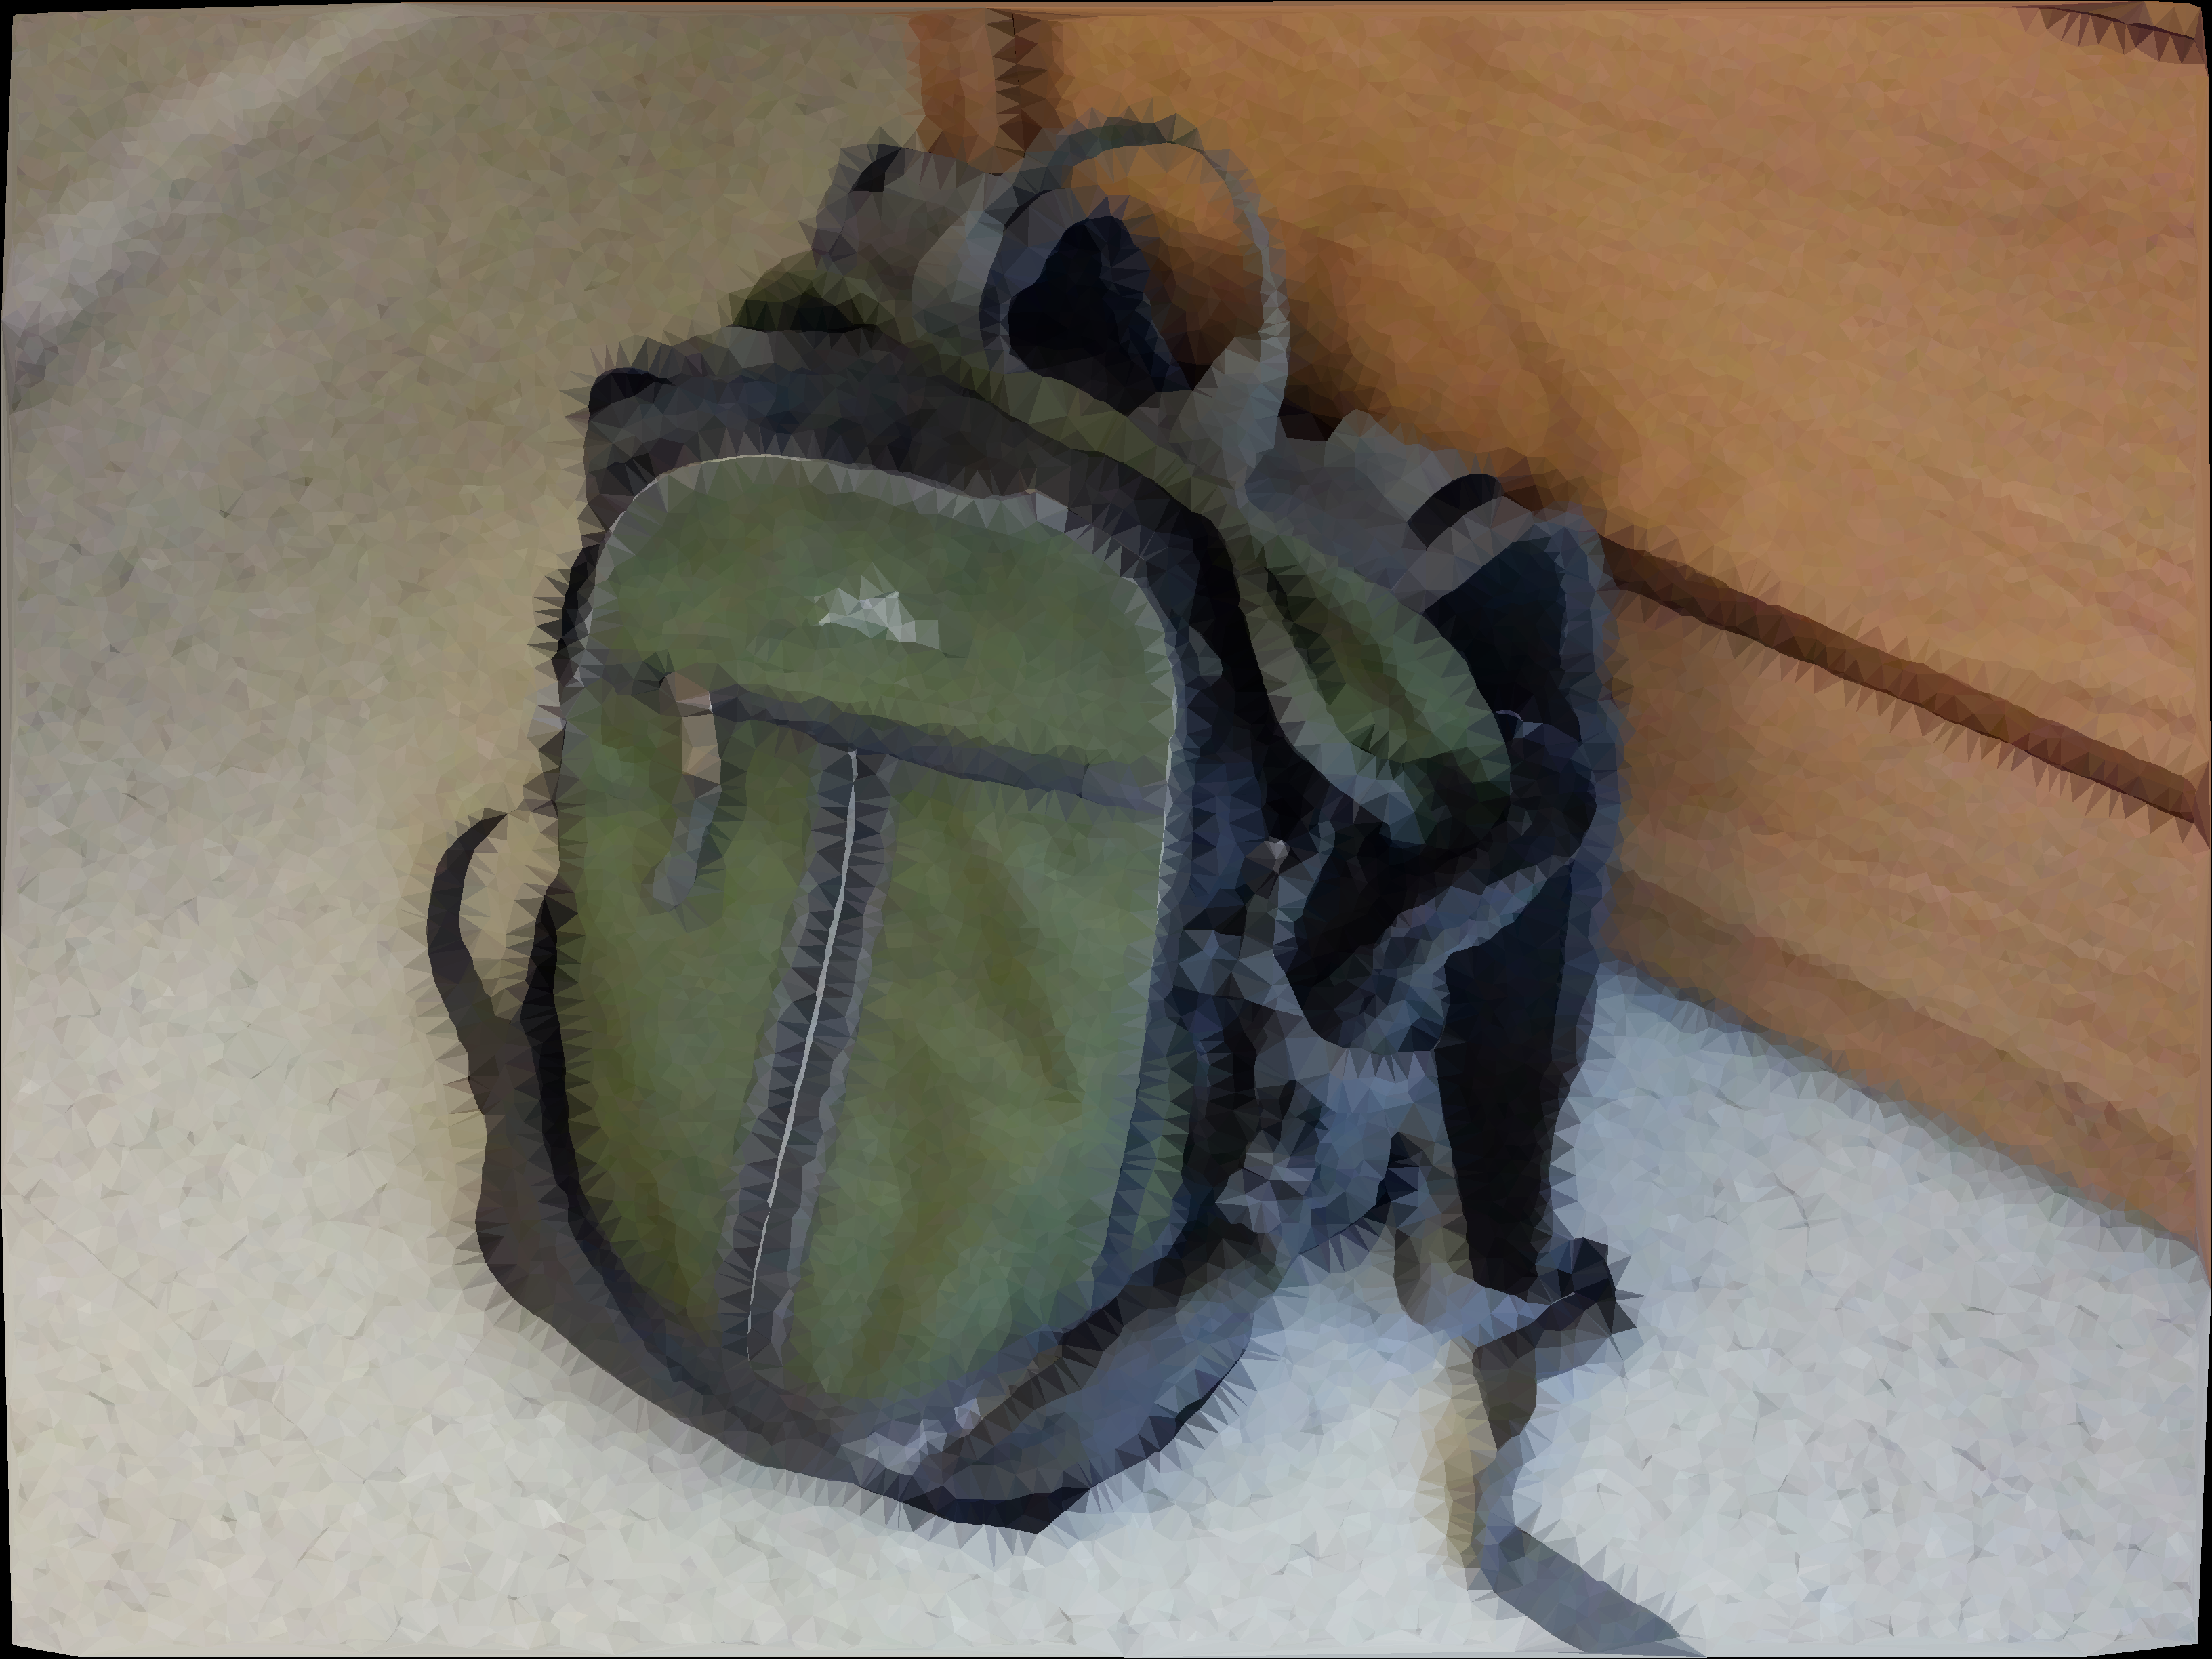
\includegraphics[width=3in]{images/delaunay}
  \caption{Delaunay triangulation of semi-dense feature points visualized
      by filling triangles with their average pixel intensity.}
  \label{fig:delaunay}
  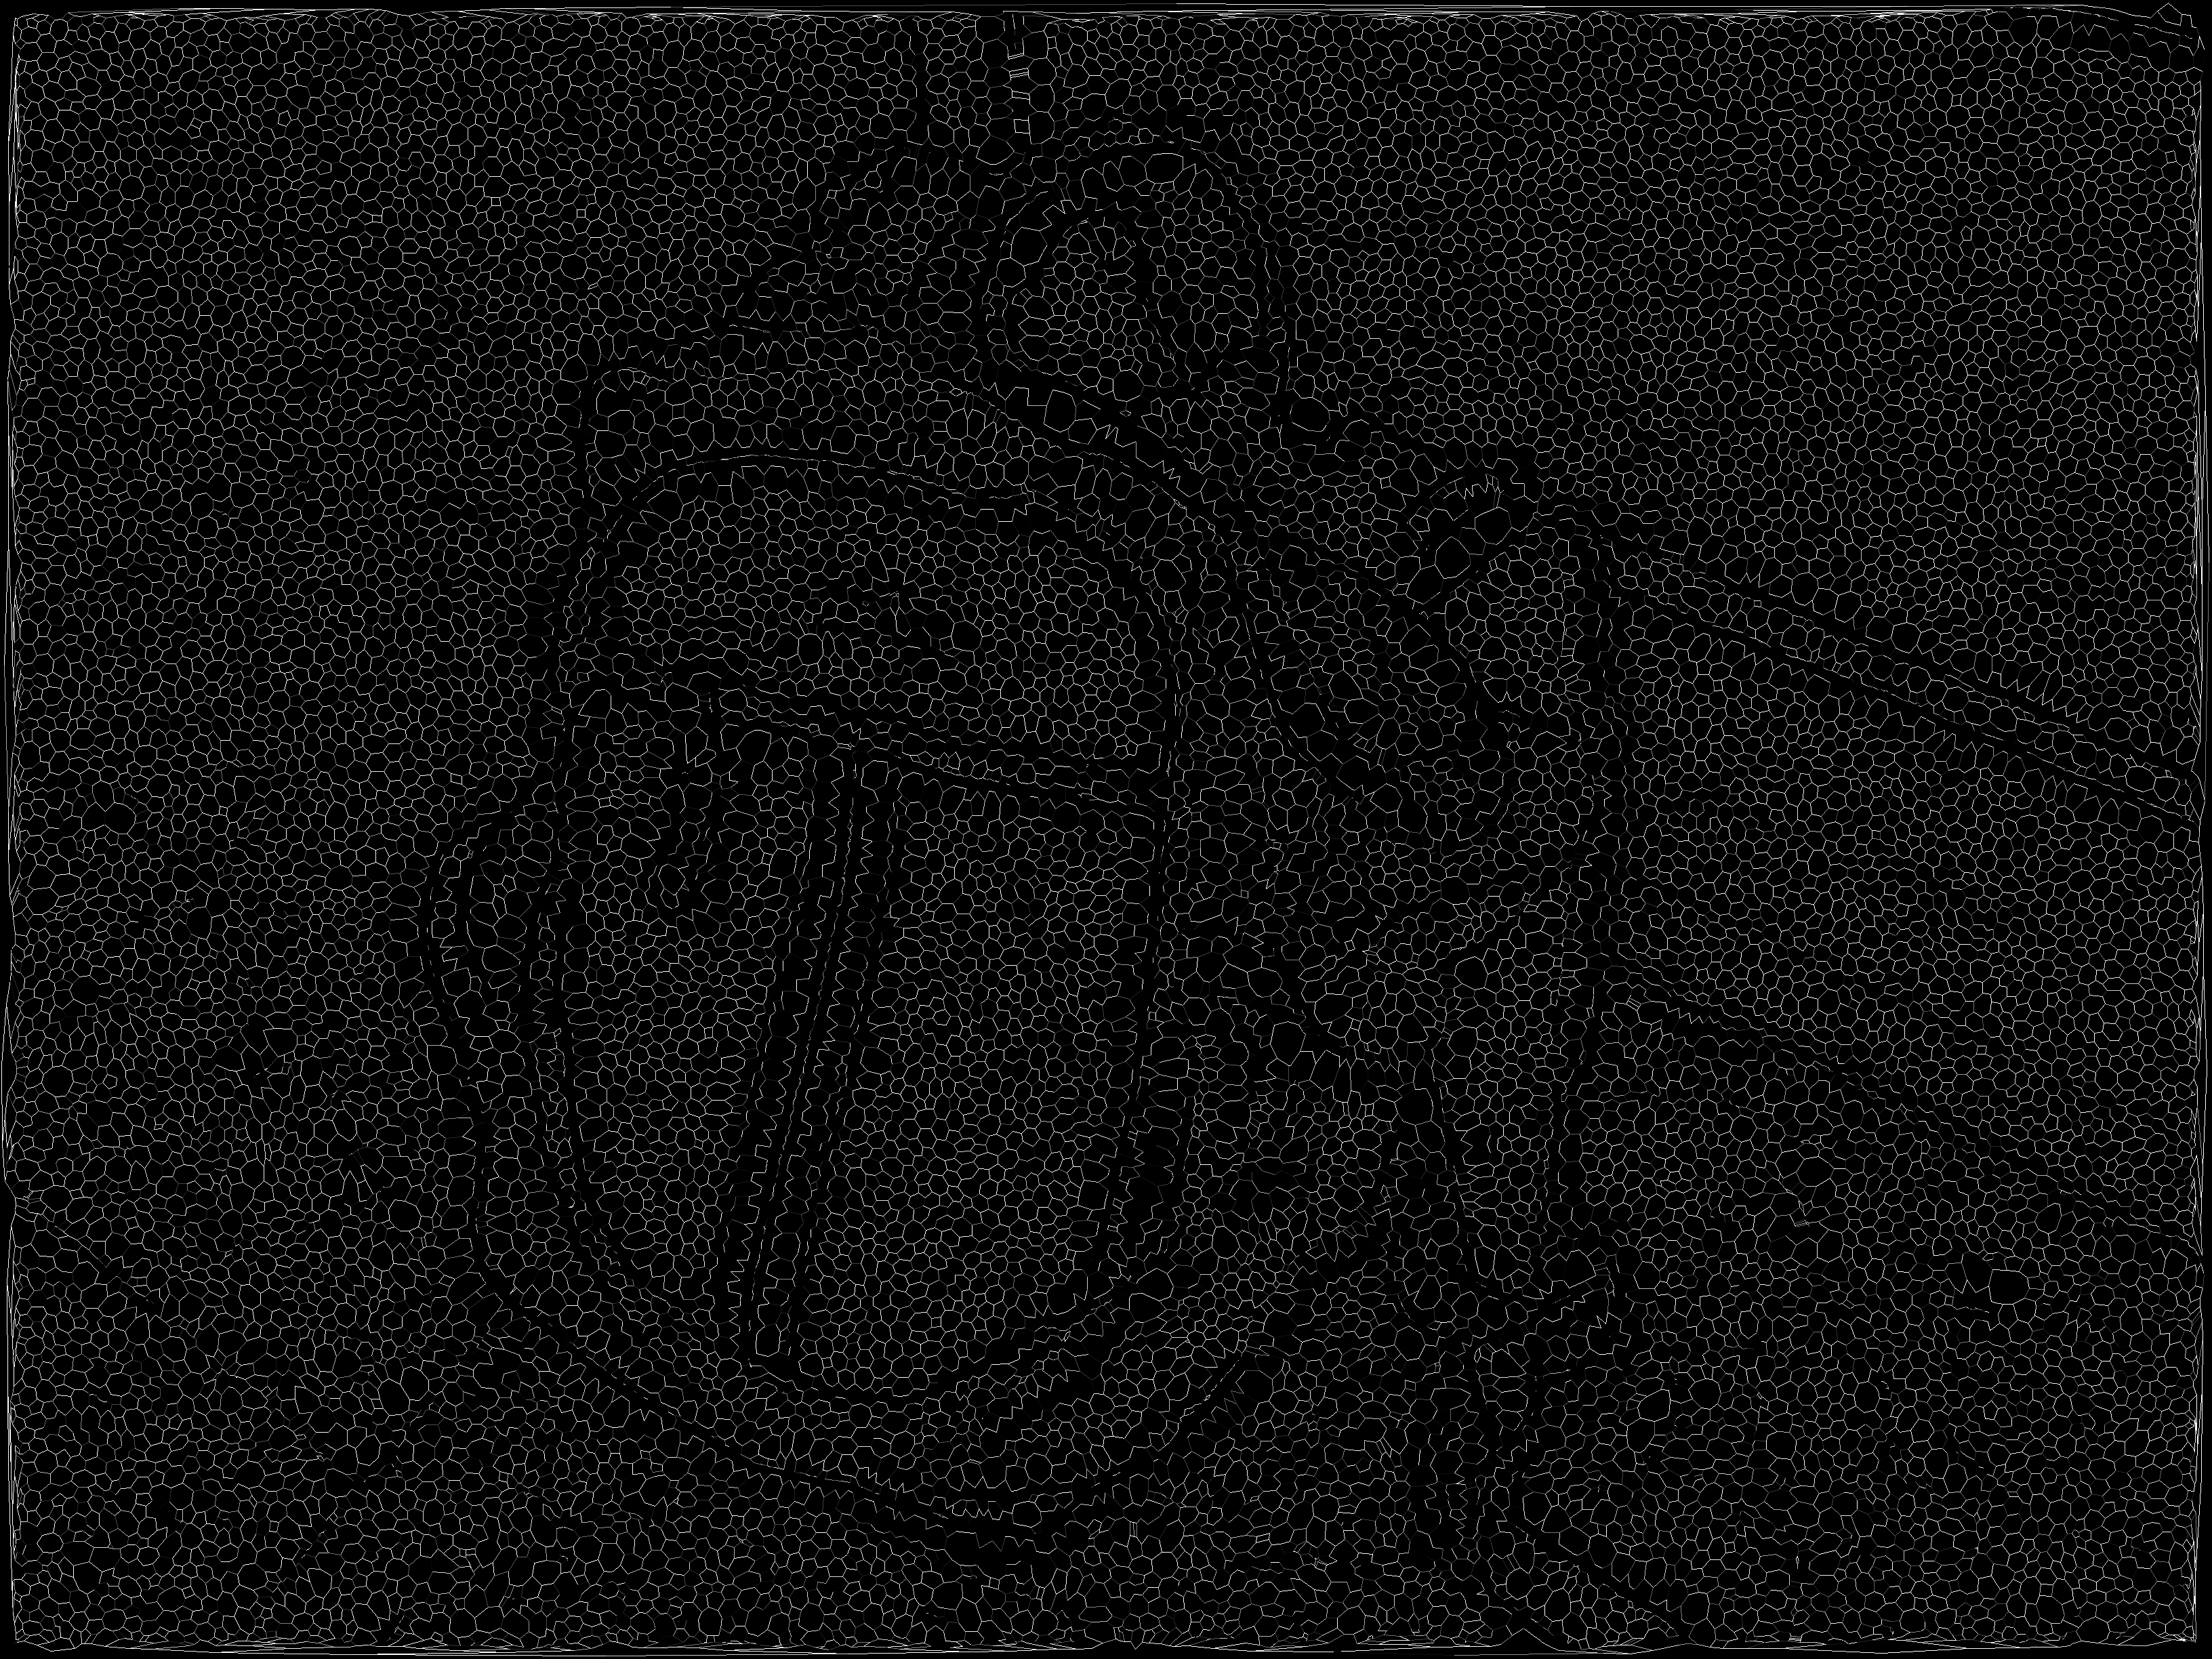
\includegraphics[width=3in]{images/delaunay_edges}
  \caption{Triangle segment edge weights depicted with brighter lines
  indicating greater edge weight.  Notice the lack of edge weights
  between triangular segments with different colors.}
  \label{fig:delaunay_edges}
\end{figure}

To begin, a delaunay triangulation is computed from the dense KLT samples
for the primary image in the sequence.
Figure~\ref{fig:delaunay} depicts one such resulting delaunay triangulation.
Note that feature points tend to lie along image edges.  Thus, the
delaunay triangulation provides a compact representation similar
to that provided by more computationally-expensive and irregular
superpixelization methods.

An undirected, weighted graph of adjacent triangles,
$G_{tri} = (V_{tri}, E_{tri})$, is then constructed
where the pairwise weight of adjacent triangles, $W(i, j)$, is determined by

\begin{equation}
    W(i, j) = \exp \left(
        \dfrac{-(\beta(C_i, C_j))^2}
        {
            \left(
                \frac{
                    (\sum_{(a, b) \in E_{tri}} \beta(C_a, C_b)^2)
                }
                {
                    |E_{tri}| - 1
                }
            \right)
        }
    \right)
\end{equation}

where $\beta$ is the Bhattacharyya distance \cite{bhattacharyya1946measure}
and $C_x$ is a trivariate normal distribution of pixel color, in the Lab color
space, of pixels in triangle $x$, estimated assuming independence between color
channels. Figure~\ref{fig:delaunay_edges} depicts the intensity of edge weights
for the triangle graph constructed for one image.

Given this delaunay triangulation and weighted edge graph, the system
then assigns a depth value to each triangle using a probabilistic model.
A markov random field is formulated consisting of a hidden state
for each triangle which may take, as possible values, any of the depth
estimates at each of the three corresponding vertices.
The probability of a particular assignment of depths to triangles is
defined to be the product of joint probabilities of adjacent triangles
as follows

\begin{equation}
    \label{eq:mrf}
    P(depth |G, W) = \frac{1}{Z} * \prod_{(i, j) \in E_{tri}}
        e^{-|depth_i - depth_j| * W(i, j)}
\end{equation}

where $Z$ is a normalization constant.

By taking the negative log of this expression
and ignoring the constant normalization coefficient, the
following energy function is derived, which is
minimized using the method of Quadratic Pseudo-Boolean Optimization (QPBO)
of \cite{rother2007optimizing} to iteratively fuse
candidate depth estimates, proposed by triangulation
using each secondary image, to the final solution
in a procedure similar to the method of alpha-expansion
described by \cite{boykov2001fast}.

\begin{equation}
    \label{eq:mrf}
    P(depth |G, W) = \sum_{(i, j) \in E_{tri}}
    \left(
        |depth_i - depth_j| * W(i, j)
    \right)
\end{equation}

Note that to compensate for the existence of feature points
for which no correct depth estimate exists from any
secondary image, a final fusion step is performed
using the median depth of adjacent triangles with
the greatest color similarity. The resulting depth
assignment can be seen in Figure~\ref{fig:qpbo_triangle_depth}.

\begin{figure}[ht]
  \centering
  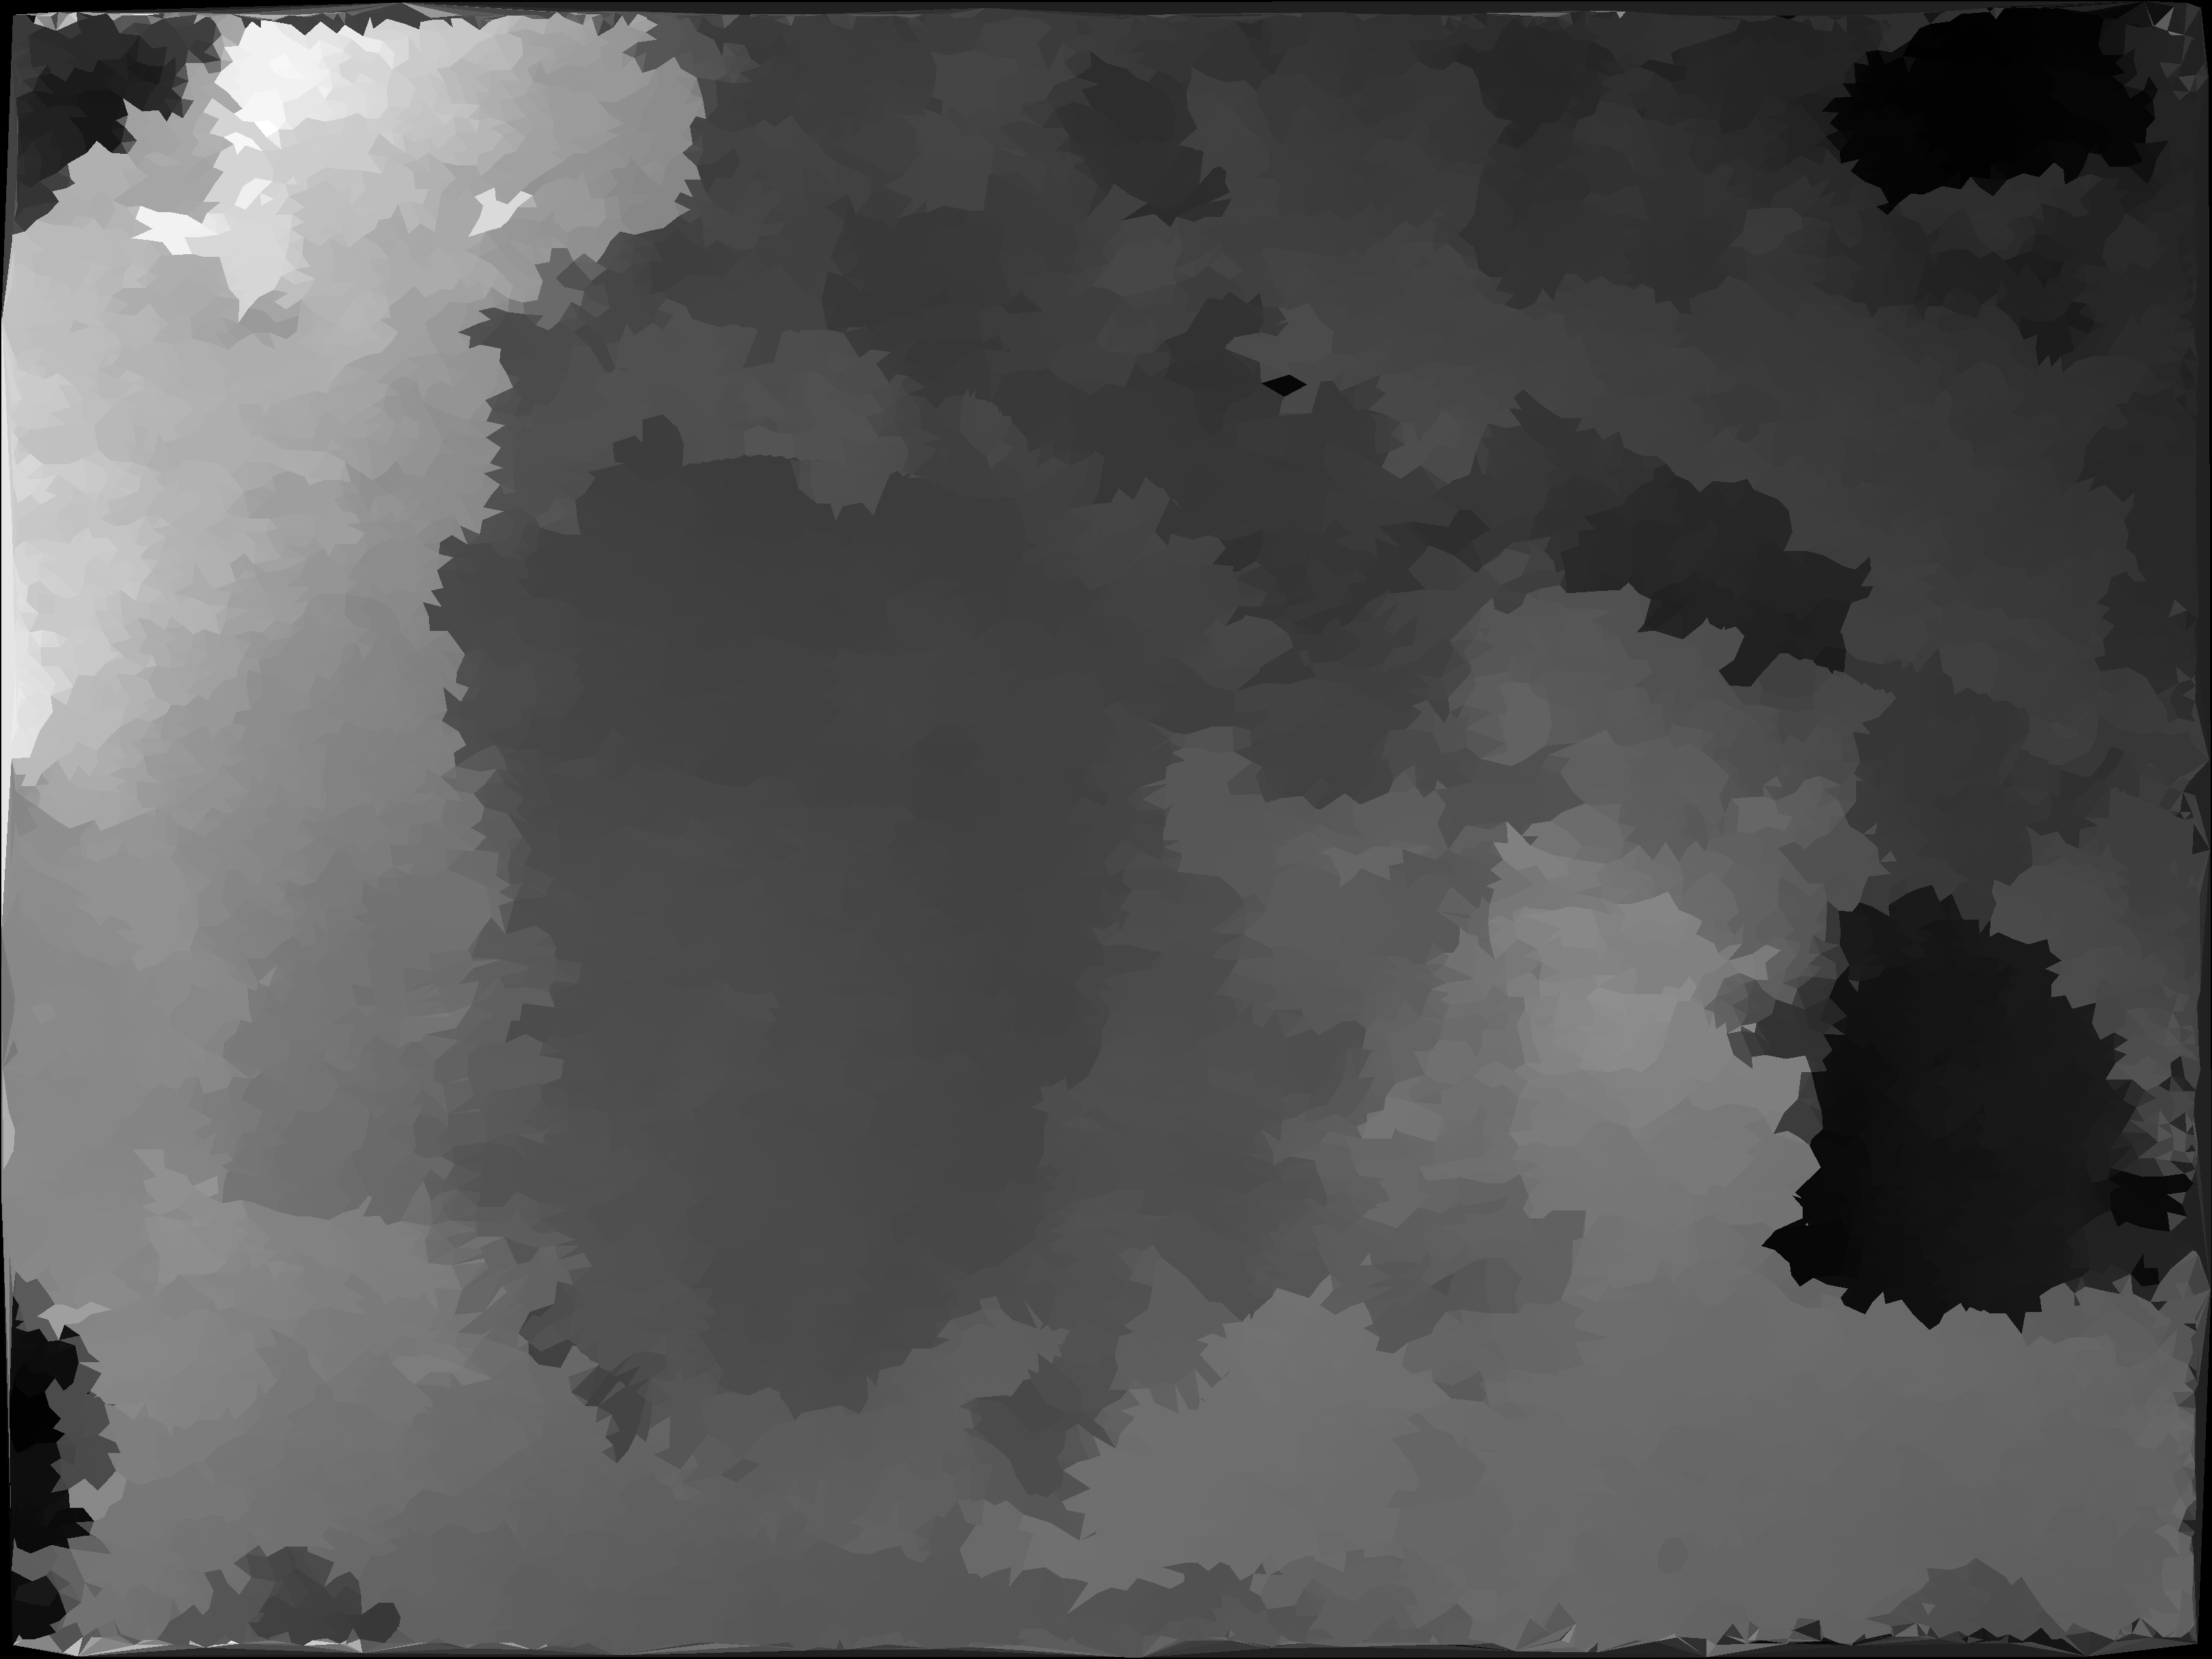
\includegraphics[width=3in]{images/qpbo_triangle_depth}
  \caption{Result of QPBO-based depth fusion.  Brighter 
  values indicate greater distance from the camera.}
  \label{fig:qpbo_triangle_depth}
  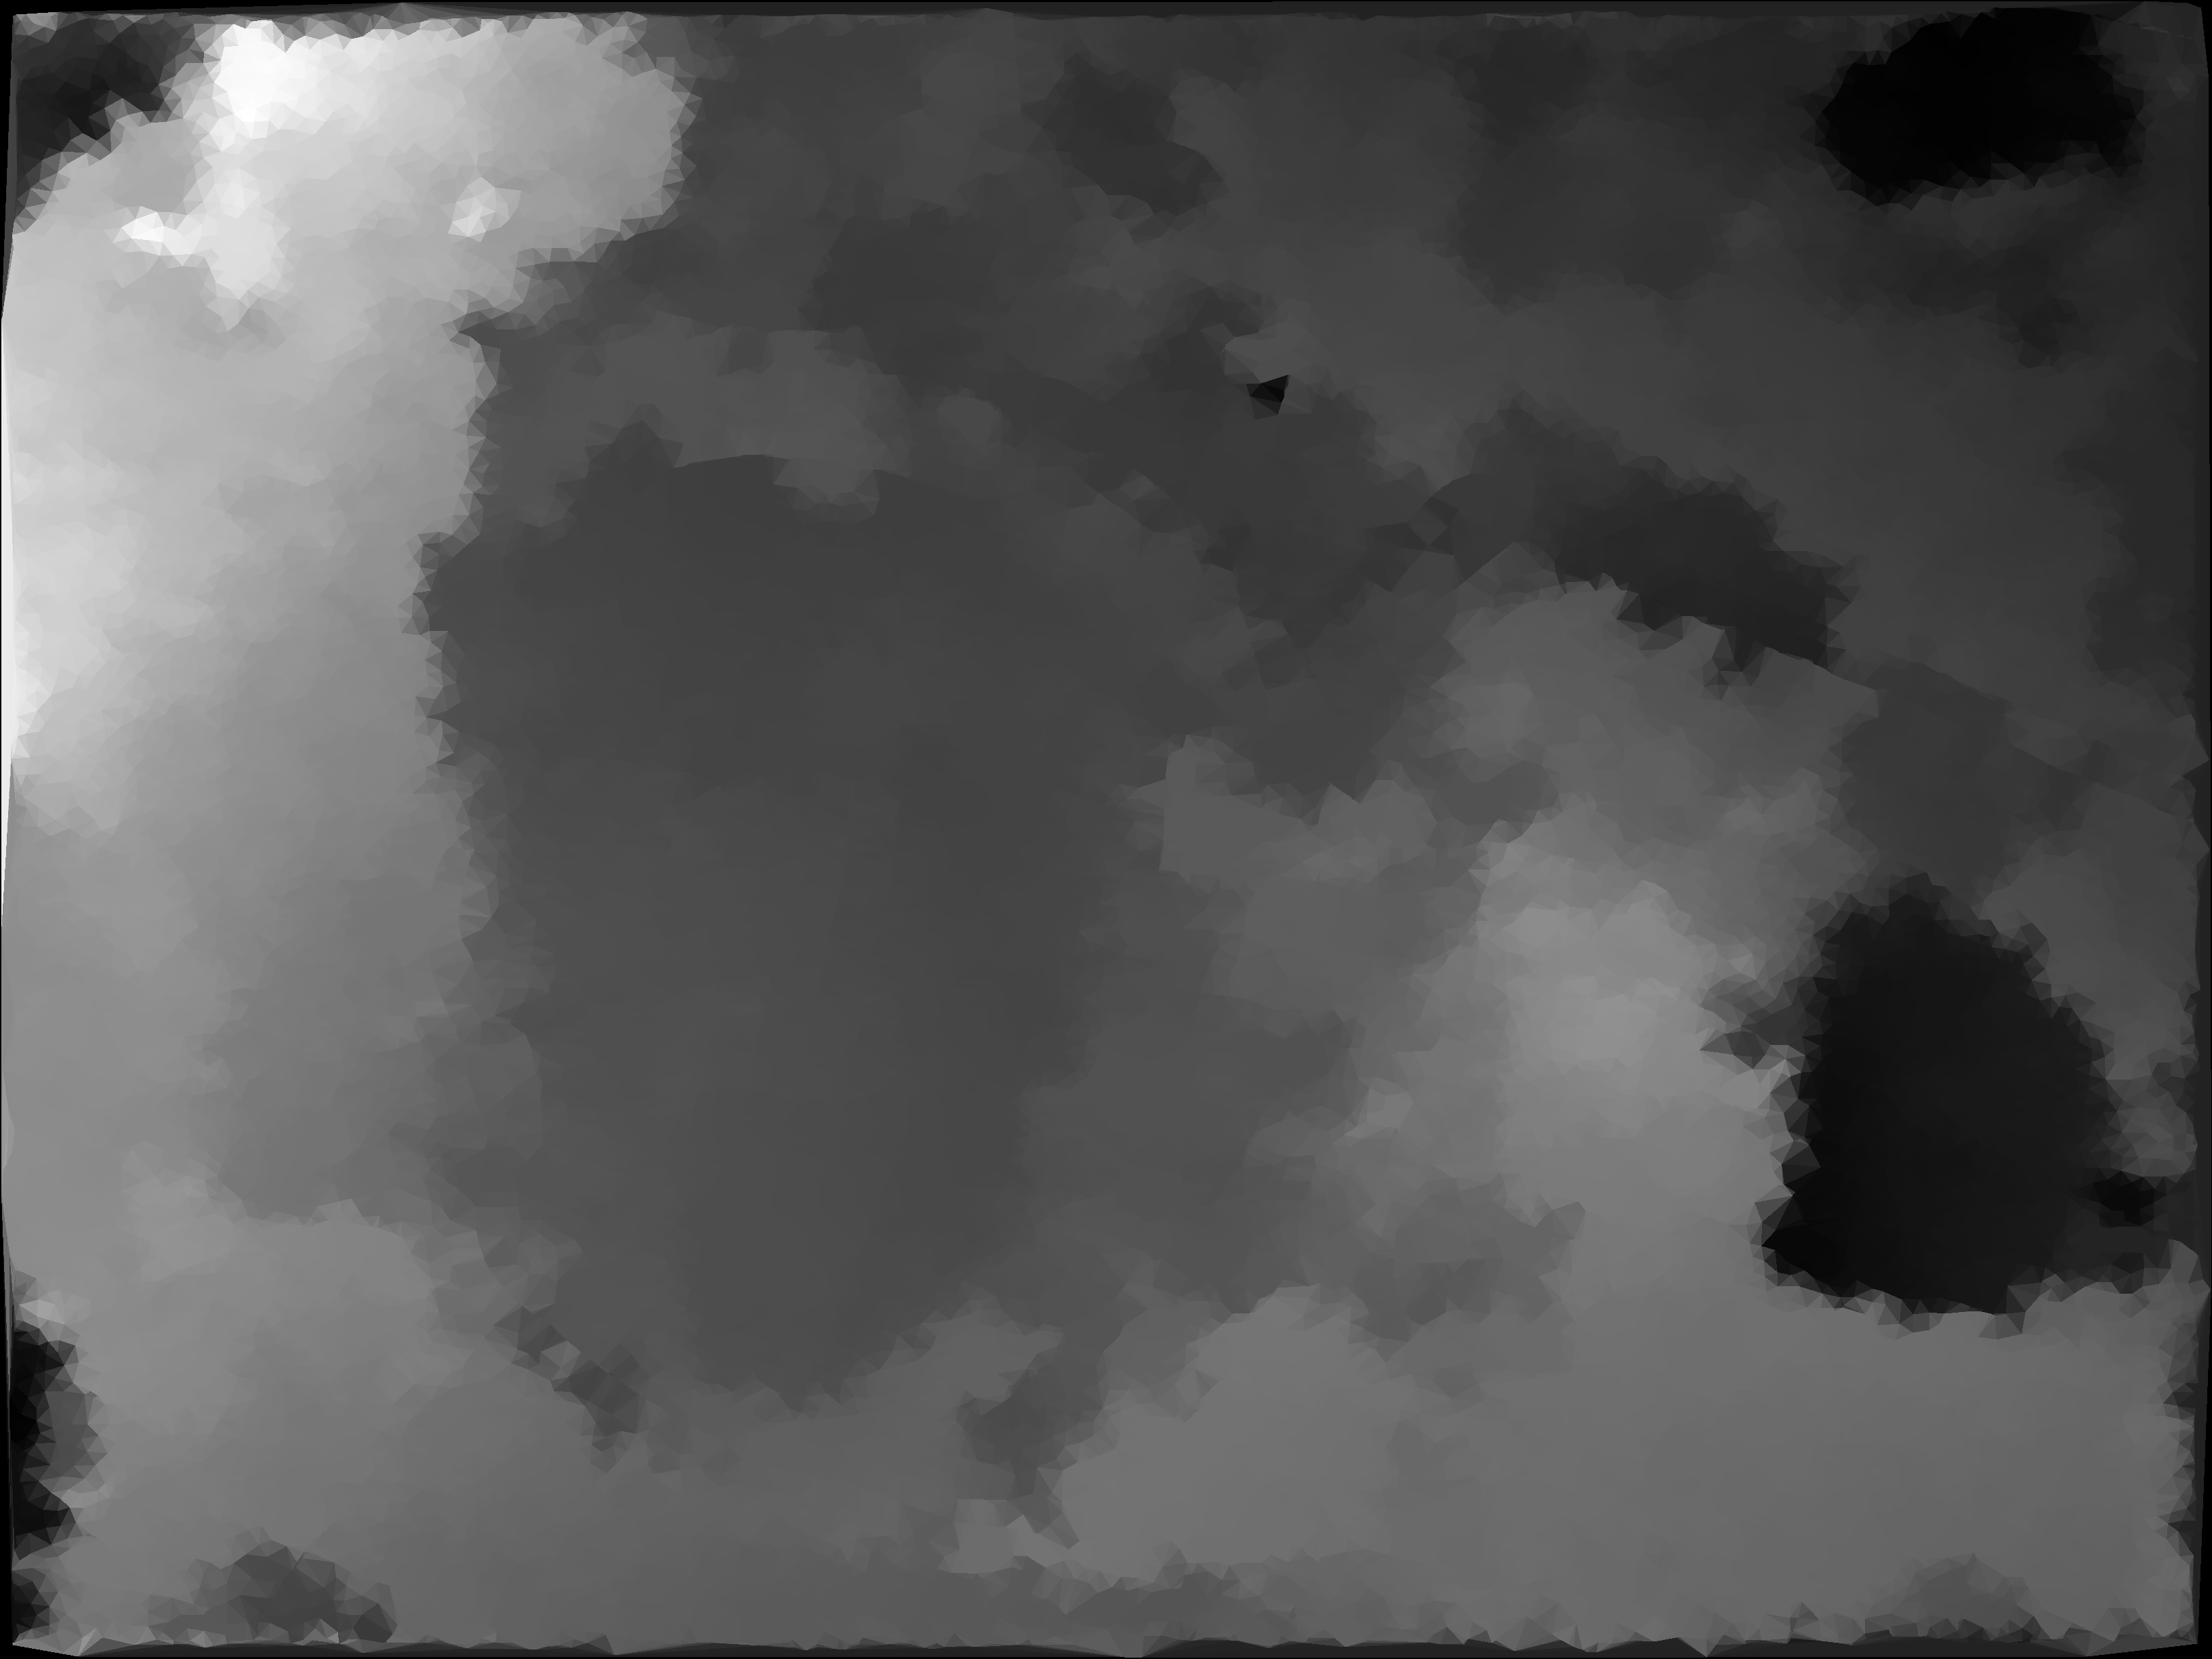
\includegraphics[width=3in]{images/qpbo_smoothed_triangle_depth}
  \caption{Result of edge-aware depth smoothing.  Brighter 
  values indicate greater distance from the camera.}
  \label{fig:smooth_triangle_depth}
\end{figure}

% Smoothing
Finally, depth values are smoothed via an iterative edge-preserving
operation using a weighted average of adjacent triangle values.
That is to say that the next depth assigned to a particular triangle, $depth_i^{t+1}$,
is computed from the current depth, $depth_i^t$, as

\begin{equation}
    \label{eq:smoothing}
    depth_i^{t + 1} = \dfrac{
        \sum_{j \in N(i)}
        \left(
            depth_j^{t} * W(i, j)
        \right)
    }
    {
        \sum_{(i, j) \in E_{tri}}
            W(i, j)
    }
\end{equation}

where $N(i)$ denotes the set of triangles neighboring triangle $i$.

Figure~\ref{fig:smooth_triangle_depth} shows the result of this smoothing
operation on a depth map.

\subsection{Rendering}


% TODO show rendered images

% Talk about rendered images

% Also talk about limitations.

\section{Conclusion}

In this paper, I have described the implementation of a system for
reconstruction of a planar representation of dense depth maps from multiple images
with an application to image-based rendering.

\begin{figure}[ht]
  \centering
  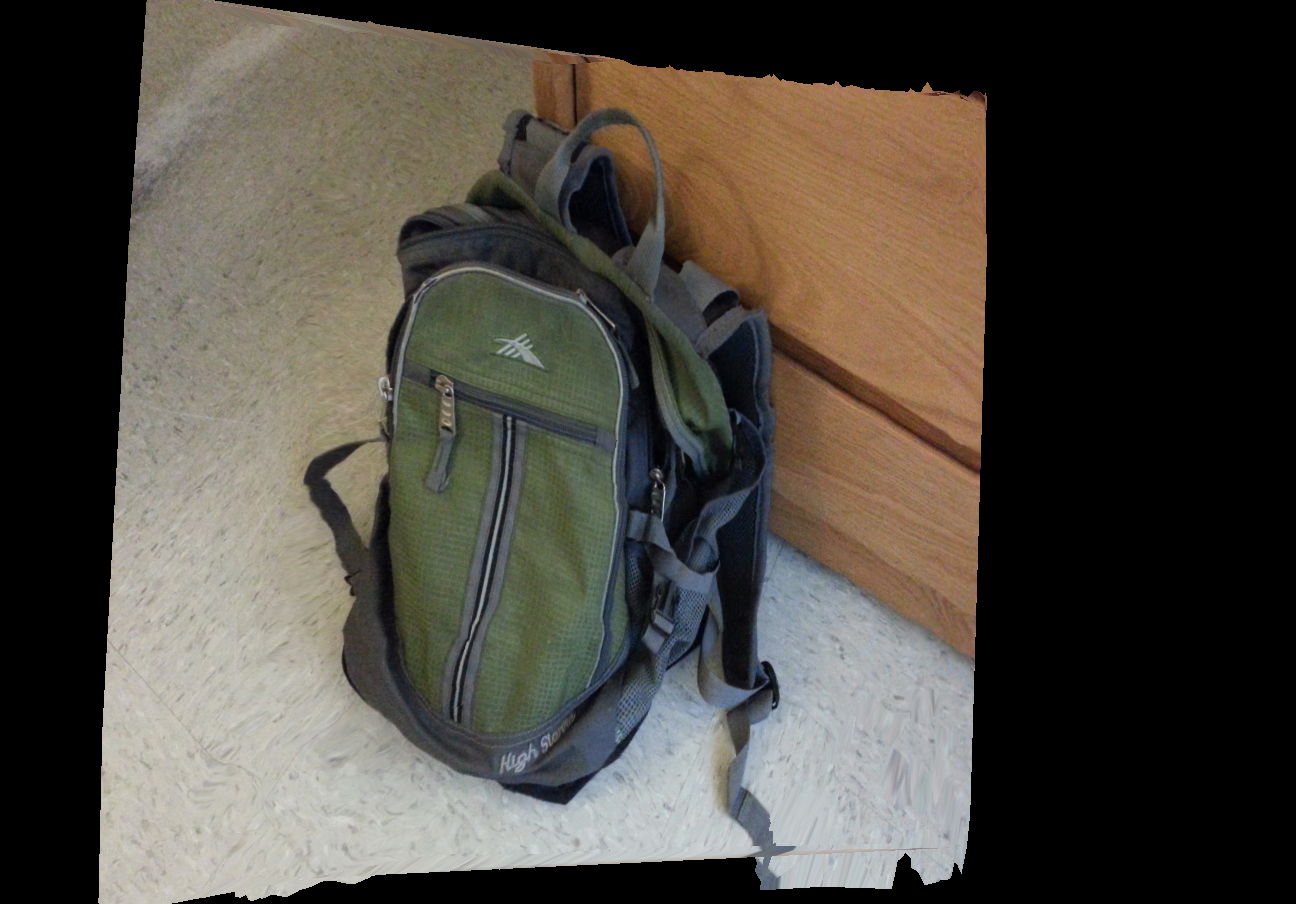
\includegraphics[width=2in]{images/r1}
  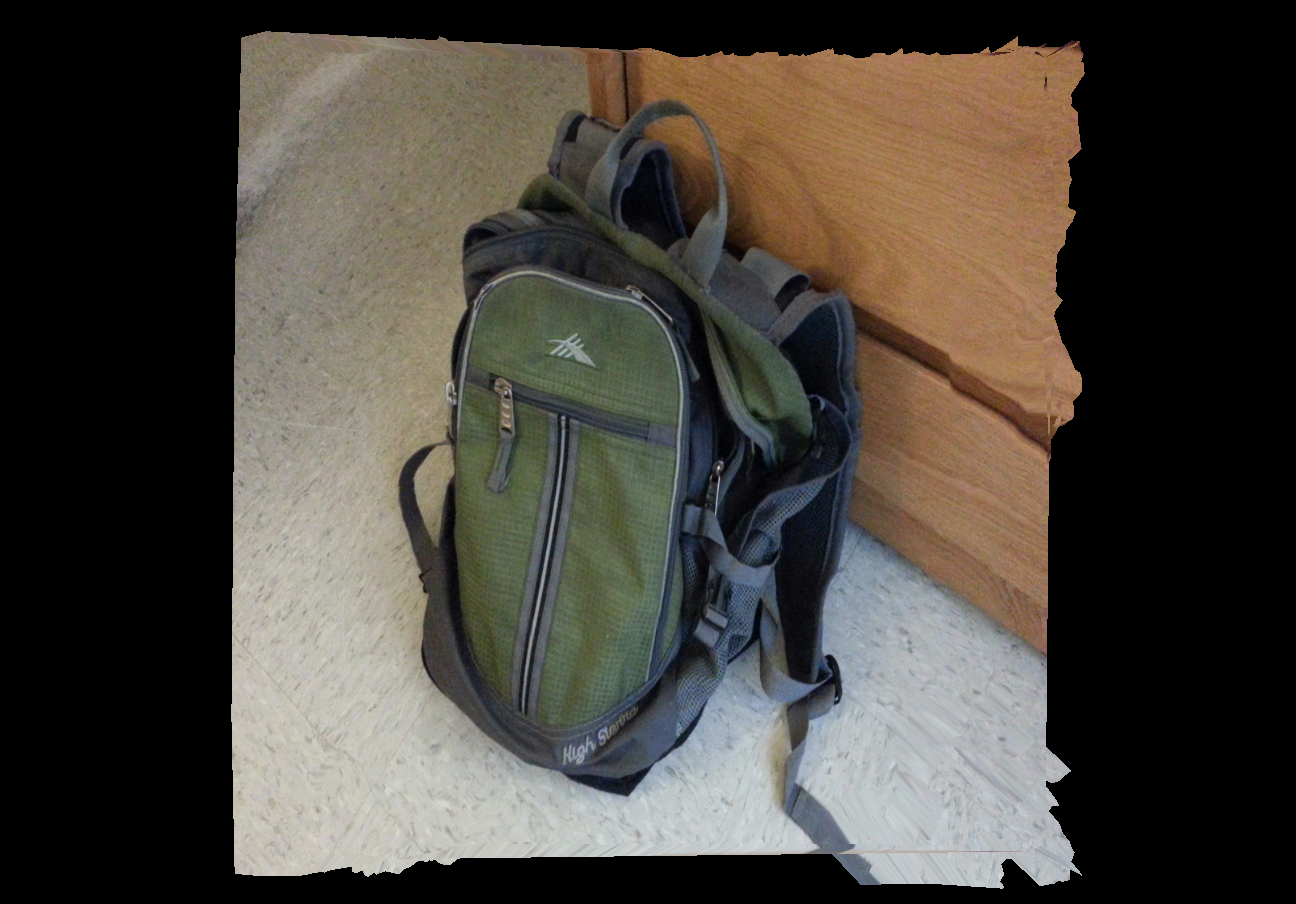
\includegraphics[width=2in]{images/r2}
  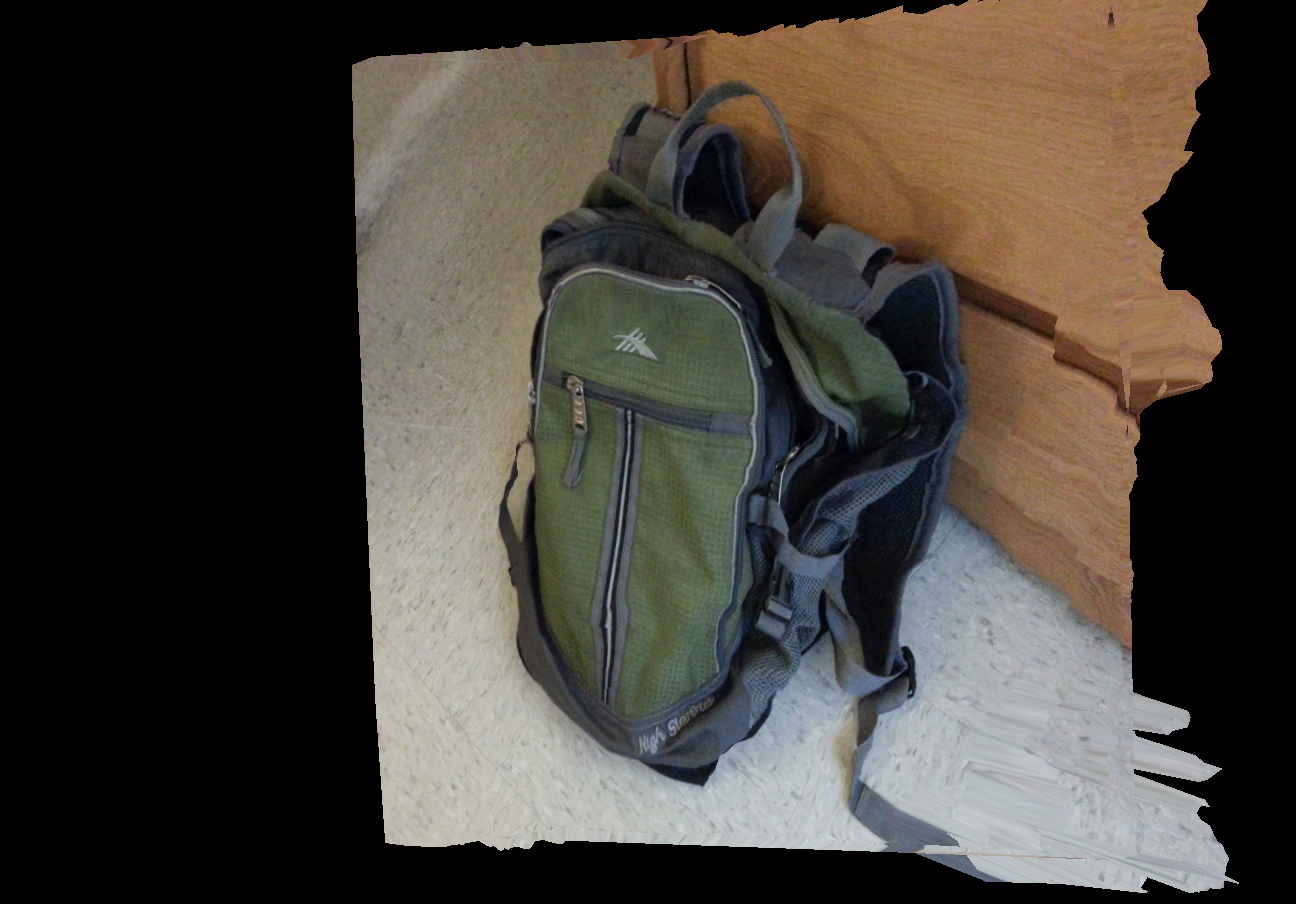
\includegraphics[width=2in]{images/r3}
  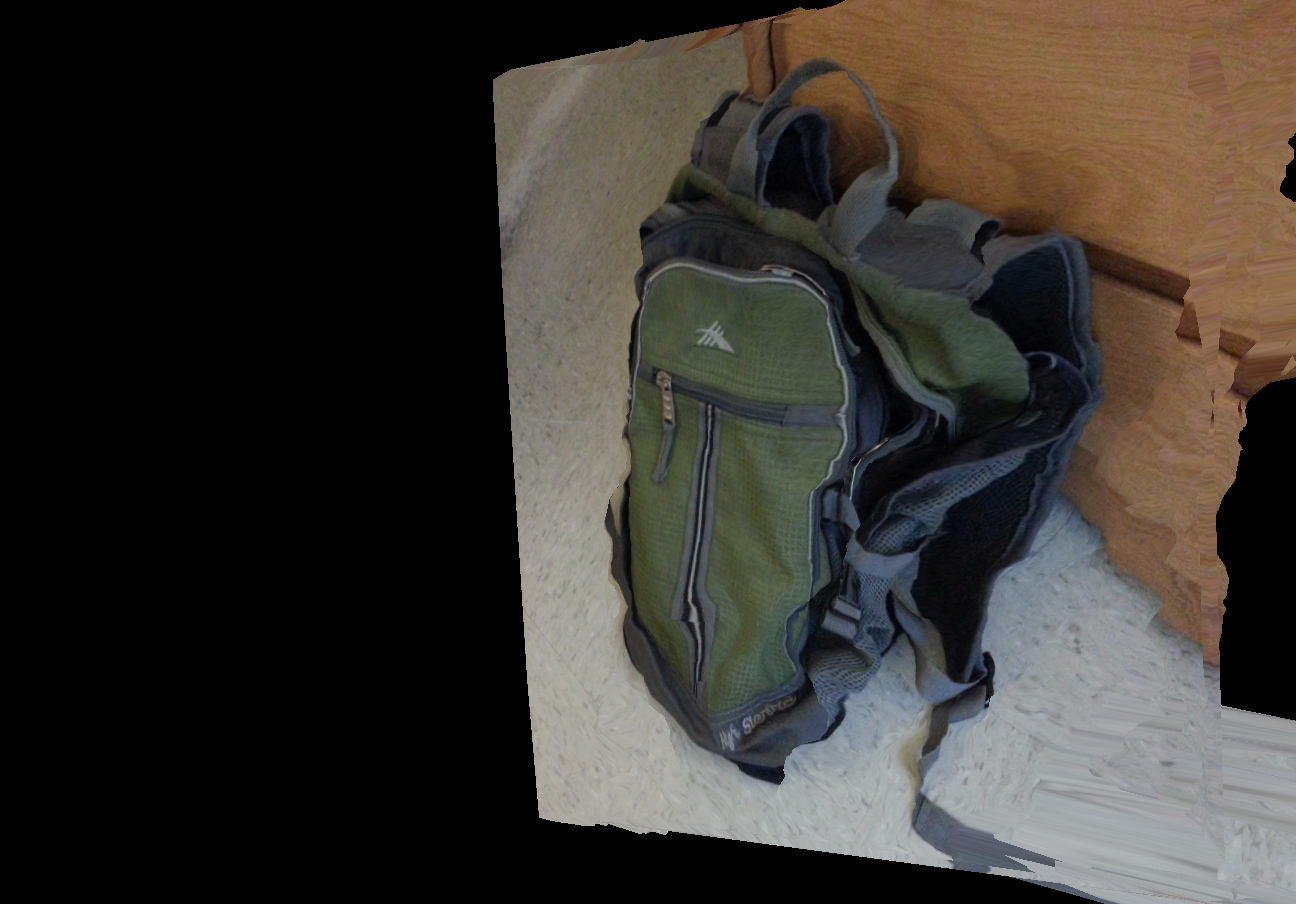
\includegraphics[width=2in]{images/r4}
  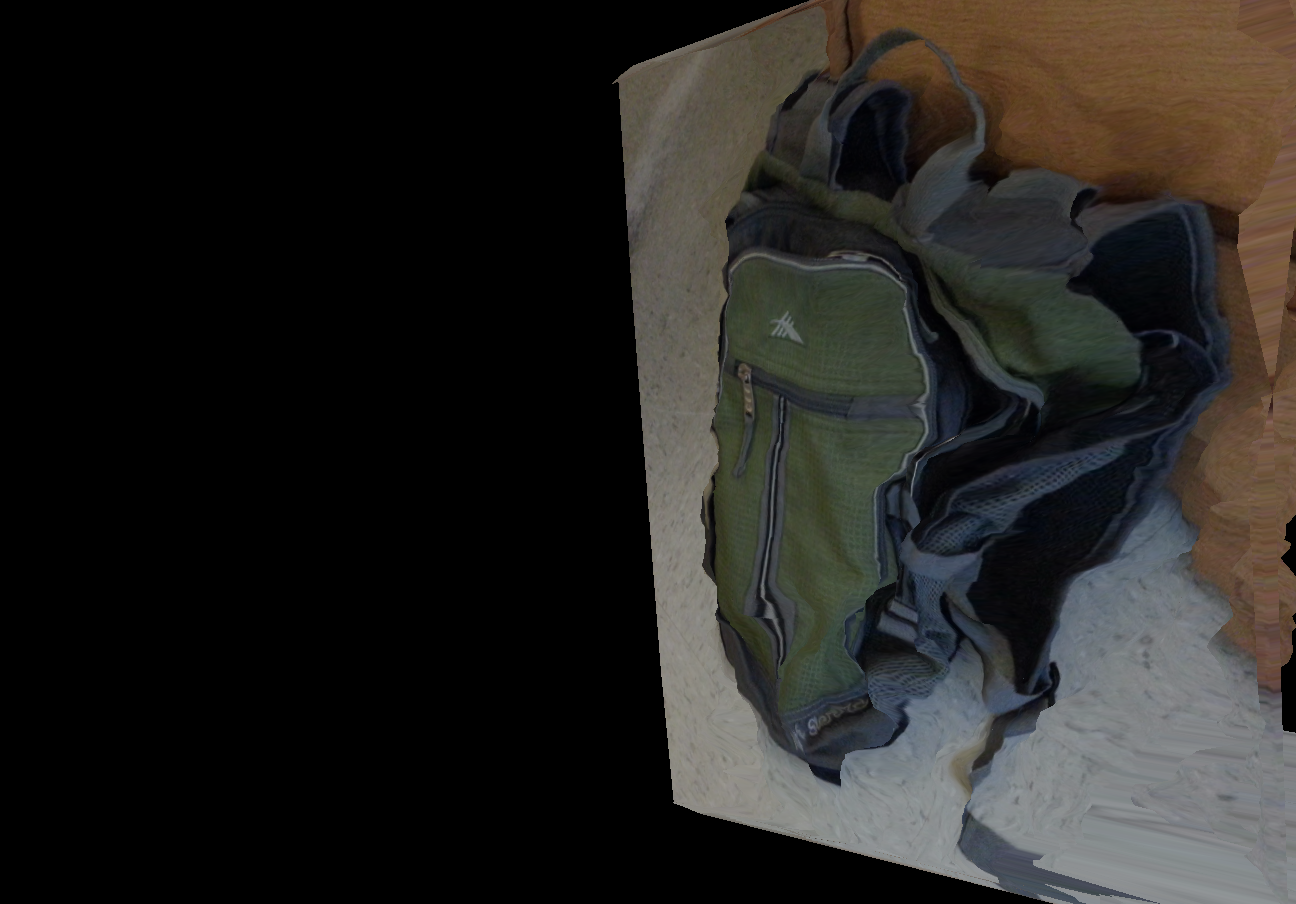
\includegraphics[width=2in]{images/r5}
  \caption{Depth-based rendering from several different orientations.}
  \label{fig:rendering}
\end{figure}

% TODO

\bibliographystyle{acmsiggraph}
\bibliography{template}
\end{document}
